End-effector velocity control (EEVC) is the act of moving your manipulator at a given speed through space at a given velocity.
EEVC is being looked at as the mass of the end-effector does not change.
Thus by controlling the velocity we also control the inertia.
In addition I will be exploring EEVC as it pertains to manipulating objects.
Through my research I have found that end-effector velocity control can be broken up into four major categories:
\textit{Time and location sensitive}, \textit{location sensitive}, \textit{time sensitive}, and \textit{time and location insensitive}.\\


\noindent \textbf{Time and Location Sensitive}: 
If your velocity control is time and location sensitive it means that your end effector needs to have a given velocity at a specific time in a specific location or the task fales.
Hitting a baseball with a bat is an example of \textit{time and location sensitive}  EEVC.
If the bat has the correct velocity but not at the correct time it will not hit the ball or the ball will not go in the desired place.  
The same goes for if it does not have the correct location but does have the correct velocity.
It is important to note that the manipulator only has instantaneous control over the object at the instant of contact.
Other examples include playing the piano, hitting a tennis ball with a racquet, a moving soccer ball with a foot or any other task that requires to \textit{hit} a \textit{moving} object.\\


\noindent \textbf{Location Sensitive}:
If your velocity control is location sensitive it means that it only matters that the velocity occurs at a given location.
The time it takes to reach that velocity will not effect the results.
Hitting a nail with a hammer is a prime example of location sensitive EEVC.  
The nail is not moving but it does need to be hit in a given location with a given velocity.
The vector of the velocity is determined by the required angle the nail needs to be hit at.
In this example the nail is not time dependent and can be hit any time.
Hitting it a $t=N$ or $t=N+1$ will not effect the results.
It is important to note that the manipulator only has instantaneous control over the object at the instant of contact.
Other examples of location sensitive end-effector velocity control are hitting a golf ball with a club, hitting a pool ball with the cue, and other activities that require a given location and direction of manipulation but are not time dependent.\\


\noindent \textbf{Time Sensitive}: 
If the location were the end-effector achieves a given velocity is not required to complete the task but the time when it happens is required it is considered \textit{time sensitive} EEVC. 
This means that the end-effector can move in any region it desired as long as the end effector achieves a given velocity at a given time.
The end-effecter's velocity can be dependent on the location achieved but the location is an independent variable and the velocity is the dependent variable.
It is important to note that the manipulator control over the object during the entirety of the motion.
This typically means that the manipulator is holding the object until the release stage.
An example of this is throwing a baseball to first base to get someone out.
Throwing the ball side arm, over arm, or even underarm does not matter as long at it is released at the correct time with the correct velocity to get it ball to the first-baseman to get the runner out.
Other example of time sensitive EEVC are any other instance where an object is thrown within a given time. \\




\noindent \textbf{Time and Location Insensitive}:
If the location and the time of when the end-effector achieves a given velocity does not matter it is considered time and location insensitive.  
The end-effecter's velocity can be dependent on the location achieved but the location is an independent variable and the velocity is the dependent variable.
In this case the manipulator has control over the object until the release stage.
Examples of this would be pitching a baseball, bowling, throwing a grenade or horseshoes etc.
Throwing is an example of when the end-effector's velocity holds a higher priority over the position.  


Mechanisms with only a single degree of freedom are restricted to throwing in a plane.   2-DOF mechanisms are able to throw in $R^3$ space with the correct kinematic structure.
Such a mechanism can choose its release point or its end-effector velocity but not both.
Mechanisms containing 3 or more DOF with the correct kinematic structure are able to throw in $R^3$ and choose both the release point and the end-effector velocity simultaneously. 

In recent work Mori et al. \cite{5152525} has show his ability to control the translational velocity, angular velocity and direction in a 2-dimension plane independently with a single DOF mechanism.
The only input is torque to the manipulator.
The concept consists is to map the input torque that will change only one of the kinimatic variables and not the other two.
This map is done over a given space and thus you can independently chose your translational and angular velocity as well as direction as long as it is in the valid search space.
The manipulator and a search space example can be seen in Fig.~\ref{fig:mori}. 

\begin{figure}[thpb]
  \centering
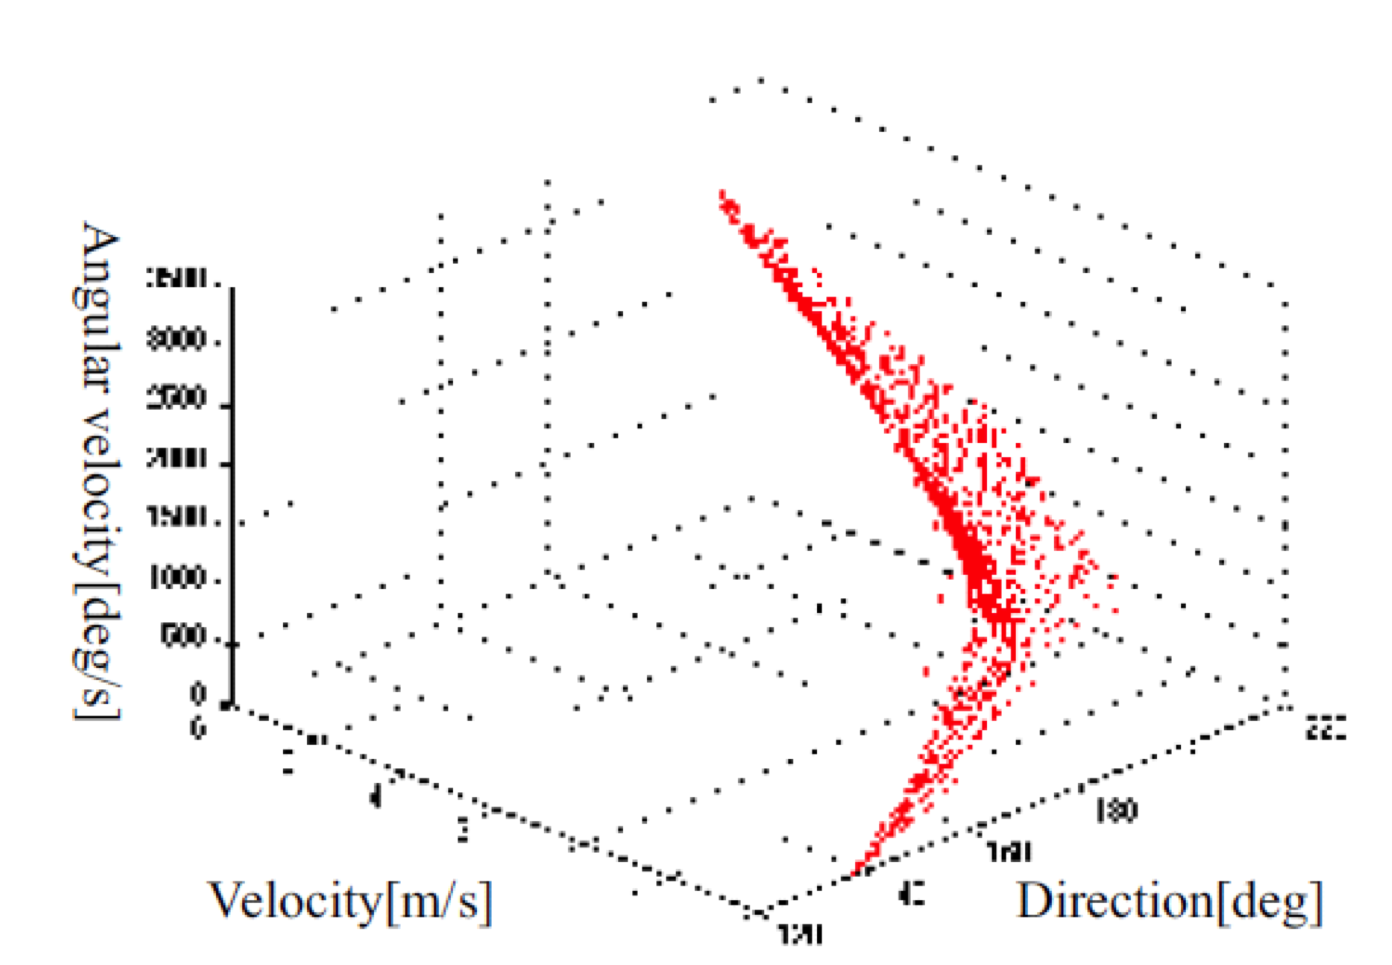
\includegraphics[width=0.4\columnwidth]{./background/pix/mori2.png}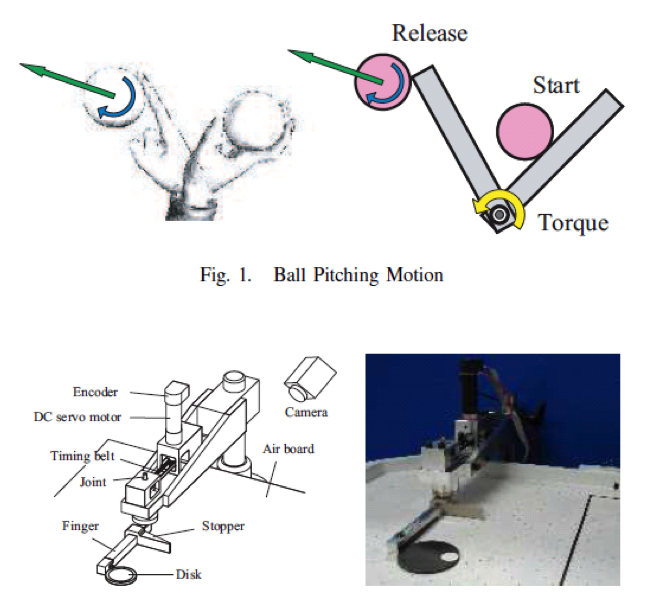
\includegraphics[width=0.4\columnwidth]{./background/pix/mori1.png}
  \caption{Map of the input torque that will change only one of the kinimatic variables and not the other two.
This map is done over a given space and thus you can independently chose your translational and angular velocity as well as direction as long as it is in the valid search space.}
  \label{fig:mori}
\end{figure}


Senoo et al.\cite{4651142} used a torque controlled 3-DOF arm to create a high speed throwing trajectory.
This arm falls into the \textit{time and location insensitive} category of throwing.
Senoo used a kinematic chain approach based on how humans throw.  
Doing this Senoo was able to achieved an end-effector velocity of 6.0 $m/s$ and can throw in $R^3$ space.
This is done via the use of a planted robot arm made by Barret Technology Inc consisting of 3-DOF with a $360^o$ rotation base yaw actuator, see Fig.~\ref{fig:senoo}. 
 

\begin{figure}[thpb]
  \centering
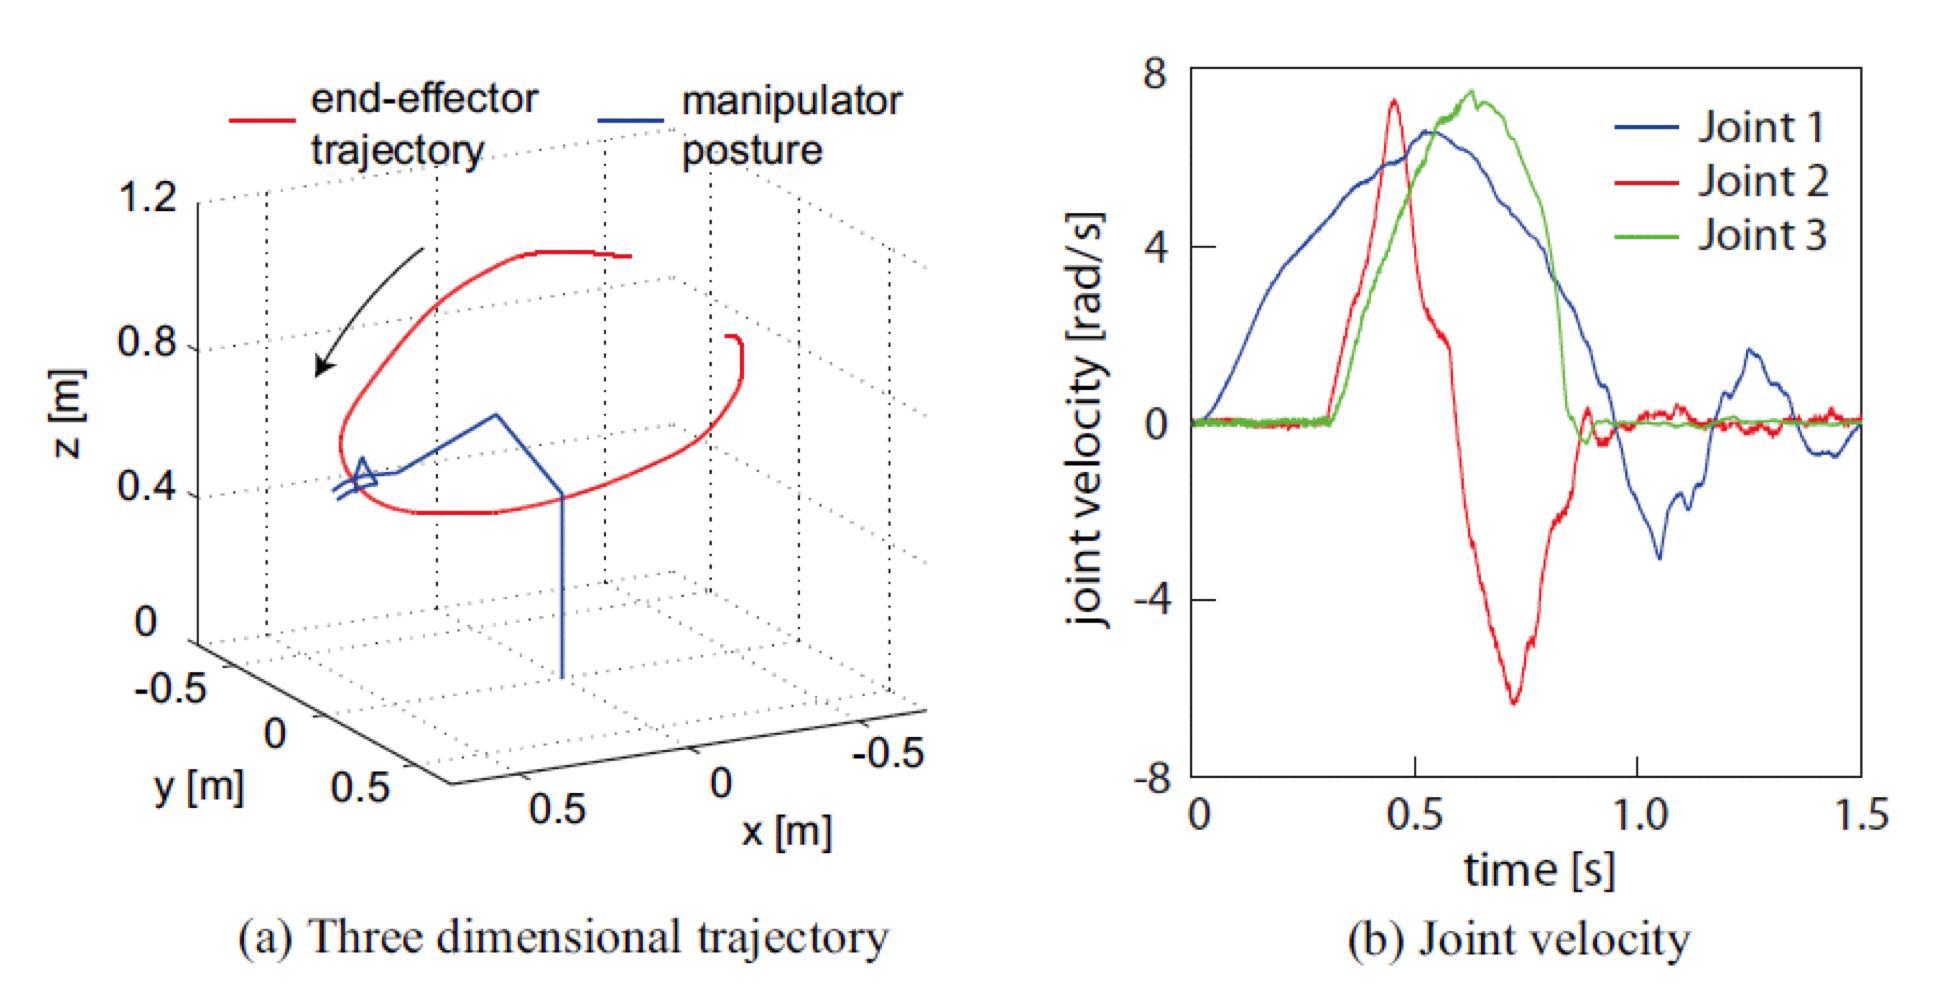
\includegraphics[width=0.6\columnwidth]{./background/pix/senoo2.png}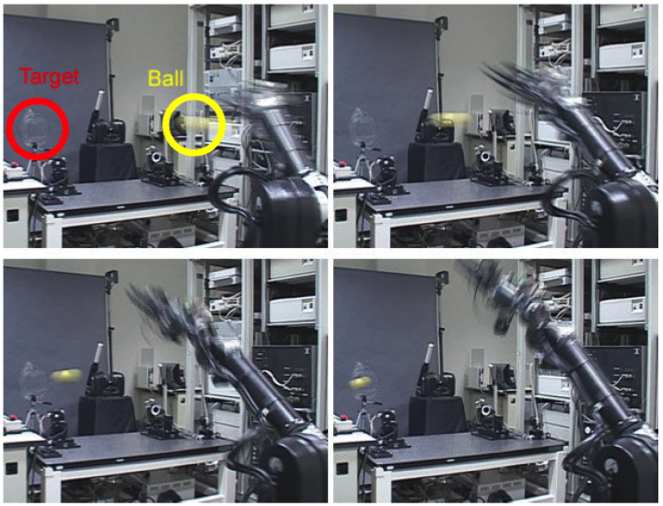
\includegraphics[width=0.4\columnwidth]{./background/pix/senoo1.png}
  \caption{3-DOF arm achieving an end-effector velocity of 6.0 $m/s$ and can throw in $R^3$ space.
This is done via the use of a planted robot arm made by Barret Technology Inc with a $360^o$ rotation base yaw actuator}
  \label{fig:senoo}
\end{figure}
 

Low degree of freedom throwing machines/robots are common.  
Typical throwing robots have between one and three degrees of freedom (DOF)~\cite{509405, Lynch97dynamicnonprehensile, 5152525, 509335, springerlink:10.1007/s10015-006-0401-0}.
All of these mechanisms are limited to throwing in a plane.   



These low degree of freedom throwing robots are either physically attached/planted to the mechanical ground or have a base that is significantly more massive then the arm.  

Haddadin et al.\cite{6094757} used their 7-DOF arm and a 6-DOF force torque sensor with standard feedback methods to dribble a basket ball.  
In addition Zhikun et al.~\cite{6094892} used reinforcement learning to teach their 7-DOF planted robot arm to play ping-pong.  
Likewise Schaal et al.~\cite{schaal01/BIRG} taught their high degree of freedom (30-DOF) humanoid to hit a tennis ball using an on-line special statistical learning methods.
Visual feedback was used in the basketball throwing robot by Hu et al.~\cite{5649335} achieving accuracy of 99\%.  
All of the latter robots were fixed to the ground to guarantee stability.

Kim et al. \cite{5686315,JooH2011438} takes the research to the next level with finding optimal overhand and sidearm throwing motions for a high degree of freedom humanoid computer model.  The model consists of 55-DOF and is not fixed to mechanical ground or a massive base.  Motor torques are then calculated to create both sidearm and overhand throws that continuously satisfies the zero-moment-point stability criteria~\cite{4309277}.  


